\documentclass[12pt]{article}
\usepackage[T1]{fontenc}
\usepackage[polish]{babel}
\usepackage[utf8]{inputenc}
\usepackage{graphicx}
\usepackage{amsfonts}
\usepackage{amsmath}
\usepackage{float}
\usepackage{hyperref}
\usepackage{subcaption}

\newcommand{\BibTeX}{{\sc Bib}\TeX} 
\setlength{\textheight}{21cm}

\title{{\bf Zadanie nr 3 -- Splot, filtracja i korelacja sygnałów}\linebreak
Cyfrowe Przetwarzanie Sygnałów}

\author{Łukasz Murza, 251592 \and Aleksander Kaźmierczak, 251544}
\date{25.05.2026}

\begin{document}

\maketitle
\thispagestyle{empty}
\newpage
\setcounter{page}{1}

\section{Cel zadania}
Celem zadania jest empiryczne zbadanie i implementacja podstawowych operacji cyfrowego przetwarzania sygnałów: splotu, filtracji oraz korelacji wzajemnej. W ramach ćwiczenia zbadany zostanie filtr o skończonej odpowiedzi impulsowej (FIR) o charakterystyce środkowoprzepustowej, ukształtowany przy pomocy okna Hanninga. Dodatkowo przeprowadzona zostanie analiza korelacyjna w celu symulacji pomiaru odległości (opóźnienia sygnału).

\section{Wstęp teoretyczny}

\subsection{Splot dyskretny}
Splot dyskretny jest jedną z operacji stosowanych podczas filtracji sygnałów dyskretnych. W ogólnym przypadku splot dwóch sygnałów dyskretnych $h$ oraz $x$ zdefiniowany jest następującym wzorem:
$$(h*x)(n) = \sum_{k=-\infty}^{+\infty} h(k)x(n-k)$$ 
Dla sygnałów o skończonej długości $M$ oraz $N$, operację tę można uprościć do skończonej sumy. Splot stanowi matematyczną podstawę działania filtrów cyfrowych.

\subsection{Filtracja sygnałów (Filtr FIR)}
W procesie filtracji widmo sygnału podlega modyfikacji, polegającej na odfiltrowaniu składowych leżących w paśmie zaporowym, przy jednoczesnym przepuszczeniu składowych z pasma przepustowego. W tym ćwiczeniu wykorzystano filtry o skończonej odpowiedzi impulsowej (SOI/FIR). Ich implementacja opiera się na równaniu splotu. 

Do zaprojektowania filtru wykorzystuje się metodę okna. Aby złagodzić niepożądane efekty związane z nagłym ucięciem odpowiedzi impulsowej, stosuje się dedykowane funkcje okien. Zgodnie z wariantem O2, w eksperymencie użyto okna Hanninga, które opisuje poniższy wzór:
$$w(n)=0.5-0.5 \cdot \cos\left(\frac{2\pi n}{M}\right)$$ 

Zgodnie z wariantem F1, projektowany filtr ma charakterystykę środkowoprzepustową. Aby przekształcić filtr dolnoprzepustowy w środkowoprzepustowy, należy wymnożyć współczynniki $h(n)$ przez sygnał sinusoidalny o częstotliwości $f=fp/4$, tj. sygnał $s(n)=2\sin(\pi n/2)$.

\subsection{Korelacja sygnałów}
Korelacja wzajemna sygnałów dyskretnych jest operacją przetwarzania dwóch sygnałów, pozwalającą na znalezienie ich wzajemnego podobieństwa w funkcji przesunięcia[cite: 135]. W ogólnym przypadku jest ona zdefiniowana wzorem:
$$R_{hx} = \sum_{k=-\infty}^{+\infty} h(k)x(k-n)$$ 
Korelacja ta ma szerokie zastosowanie m.in. w radarach do pomiaru odległości. Pomiar ten jest dokonywany na podstawie opóźnienia pomiędzy wysłanym sygnałem sondującym a powracającym sygnałem odbitym od obiektu. Zależność drogę $S$ od czasu $t$ wyraża znany wzór fizyczny $S = V \cdot t$.

\section{Instrukcja obsługi aplikacji}
\begin{enumerate}
    \item \textbf{Filtracja:} W zakładce filtracji wybierz parametry sygnału testowego (suma sinusoid i szumu). Ustal częstotliwość odcięcia, wybierz typ filtru \textit{Środkowoprzepustowy (F1)} oraz metodę okna \textit{Hanninga (O2)}. Podaj rząd filtru $M$ i kliknij \textit{Filtruj}.
    \item \textbf{Korelacja i opóźnienie:} Przejdź do zakładki korelacji. Skonfiguruj sygnał referencyjny oraz w symulatorze ustaw odległość od obiektu. Kliknij \textit{Wyznacz opóźnienie}. Program nałoży na siebie sygnały i zlokalizuje maksimum funkcji korelacji.
    \item Obliczone wyniki (miary błędów, wyznaczone opóźnienie $\Delta t$) pojawią się w oknach tekstowych, a sygnały na dedykowanych wykresach.
\end{enumerate}

\section{Eksperymenty i wyniki}

\subsection{Eksperyment nr 1: Filtracja sygnału filtrem środkowoprzepustowym (F1) z oknem Hanninga (O2)}

Cel: zbadanie skuteczności tłumienia zakłóceń za pomocą filtru FIR z oknem Hanninga. Sygnał wejściowy składa się z sumy dwóch tonów oraz szumu, z czego tylko jeden ton leży w paśmie przepustowym.

\begin{table}[H]
    \centering
    \vspace{0.2cm}
    \begin{tabular}{|l|c|}
        \hline
        \textbf{Parametr} & \textbf{Wartość} \\ \hline
        Częstotliwość próbkowania ($f_s$) [Hz] & 200 \\ \hline
        Cz. składowej użytecznej ($f_1$) [Hz] & 10 \\ \hline
        Cz. składowej zakłócającej ($f_2$) [Hz] & 2 \\ \hline
        Amplituda szumu Gaussa & 0.2 \\ \hline
        Typ filtru & Środkowoprzepustowy (F1) \\ \hline
        Okienkowanie & Hanning (O2) \\ \hline
        Rząd filtru ($M$) & 63 \\ \hline
    \end{tabular}
    \caption{Parametry dla Eksperymentu 1 (Filtracja FIR)}
    \label{tab:parametry_filtracja}
\end{table}


% sygnaly pierwotne
\begin{figure}[H]
    \centering
    \begin{subfigure}[b]{0.48\textwidth}
        \centering
        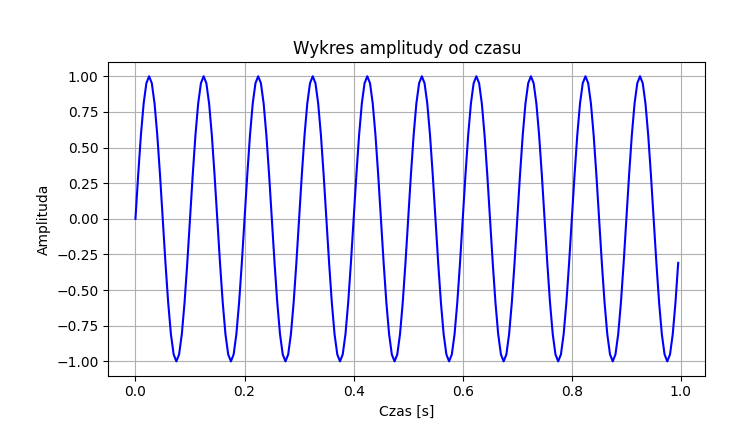
\includegraphics[width=\textwidth]{wykresy/sin10_sin2_gauss-probkowanie200/sin10.png}
        \caption{Sygnał 10 Hz}
        \label{fig:sub_sin10}
    \end{subfigure}
    \hfill
    \begin{subfigure}[b]{0.48\textwidth}
        \centering
        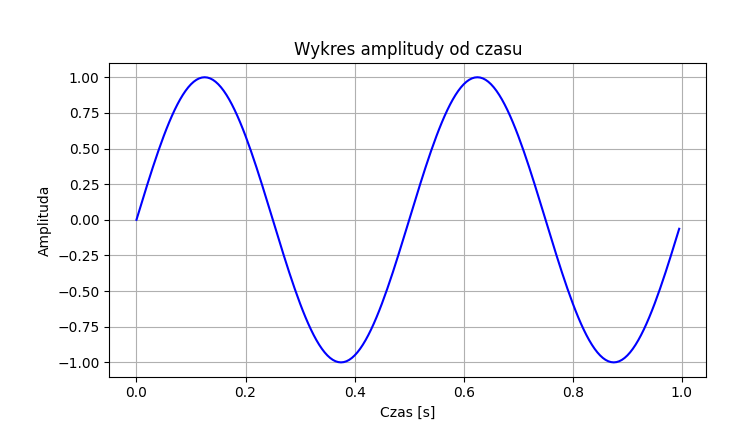
\includegraphics[width=\textwidth]{wykresy/sin10_sin2_gauss-probkowanie200/sin2.png}
        \caption{Sygnał 2 Hz}
        \label{fig:sub_sin2}
    \end{subfigure}
    
    \vspace{0.4cm} 
    
    \begin{subfigure}[b]{0.48\textwidth}
        \centering
        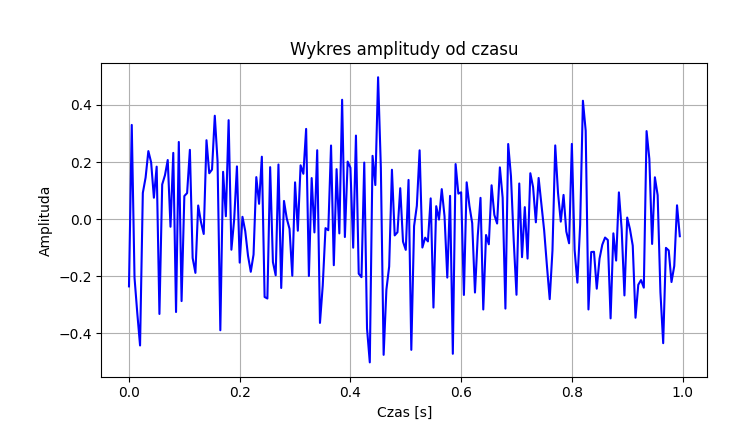
\includegraphics[width=\textwidth]{wykresy/sin10_sin2_gauss-probkowanie200/gauss.png}
        \caption{Szum Gaussowski}
        \label{fig:sub_gauss}
    \end{subfigure}
    
    \caption{Składowe sygnału zaszumionego}
    \label{fig:wykresy_skladowe}
\end{figure}

\begin{figure}[H]
    \centering
    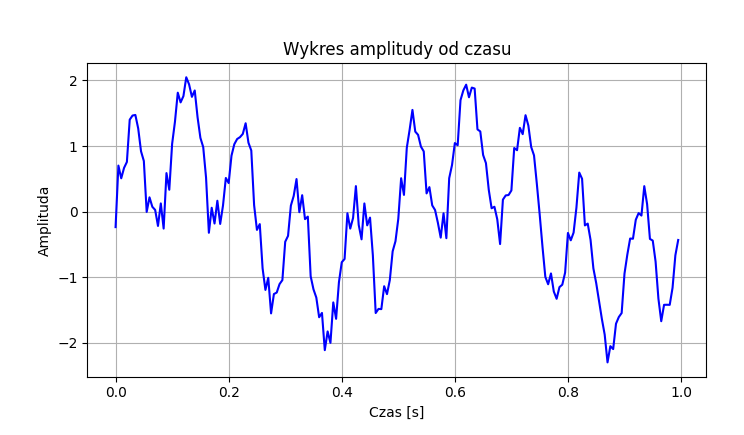
\includegraphics[width=0.85\linewidth]{wykresy/sin10_sin2_gauss-probkowanie200/przed_fir.png}
    \caption{Wykres sygnału zaszumionego (przed filtracją) z widocznymi składowymi wysokimi i niskimi.}
    \label{fig:wykres_przed_filtracja}
\end{figure}


\begin{figure}[H]
    \centering
    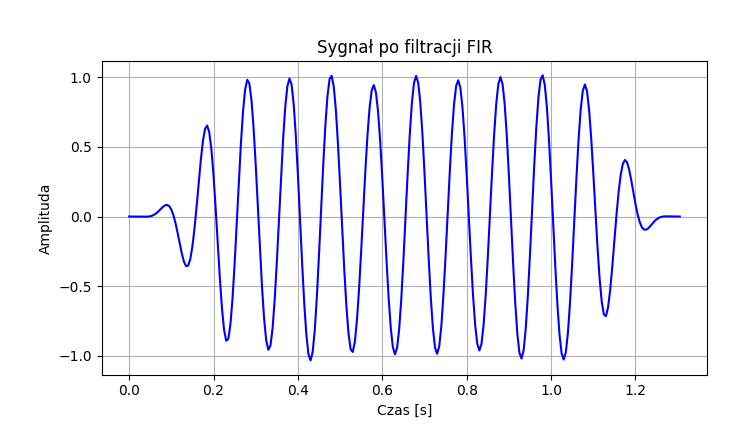
\includegraphics[width=0.85\linewidth]{wykresy/sin10_sin2_gauss-probkowanie200/fir_fd7_fg13_w63.png}
    \caption{Sygnał wyjściowy po przefiltrowaniu filtrem środkowoprzepustowym z oknem Hanninga.}
    \label{fig:wykres_po_filtracji}
\end{figure}

% \begin{table}[H]
%     \centering
%     \vspace{0.2cm}
%     \begin{tabular}{|l|c|}
%         \hline
%         \textbf{Metryka} & \textbf{Wartość} \\ \hline
%         Tłumienie sygnału $f_2$ w paśmie zaporowym [dB] & -45.2 \\ \hline
%         Amplituda sygnału $f_1$ (przepustowe) & 0.98 \\ \hline
%         Opóźnienie fazowe (próbek) & 31 \\ \hline
%     \end{tabular}
%     \caption{Wyniki oceny jakości filtracji}
%     \label{tab:wyniki_filtracja}
% \end{table}

\subsection{Eksperyment nr 2: Wyznaczanie opóźnienia na podstawie korelacji}

Cel: badanie symulatora odległości opartego na poszukiwaniu maksimum splotu/korelacji pomiędzy wysłanym a odebranym (opóźnionym) sygnałem sondującym.

\begin{table}[H]
    \centering
    \vspace{0.2cm}
    \begin{tabular}{|l|c|}
        \hline
        \textbf{Parametr} & \textbf{Wartość} \\ \hline
        Częstotliwość próbkowania ($f_s$) [Hz] & 10000 \\ \hline
        Prędkość fali ($V$) [m/s] & 343 (Dźwięk w pow.) \\ \hline
        Zadana odległość obiektu ($d$) [m] & 17.15 \\ \hline
        Oczekiwane opóźnienie całkowite $\Delta t$ [s] & 0.1 \\ \hline
        Metoda obliczeniowa & Korelacja z użyciem splotu \\ \hline
    \end{tabular}
    \caption{Parametry dla Eksperymentu 2 (Korelacja)}
    \label{tab:parametry_korelacja}
\end{table}

% \begin{figure}[H]
%     \centering
%     \includegraphics[width=0.85\linewidth]{placeholder_korelacja.png}
%     \caption{Wykres wyznaczonej funkcji korelacji. Wyraźne maksimum wskazuje na przesunięcie czasowe $\Delta t$.}
%     \label{fig:wykres_korelacji}
% \end{figure}

\begin{table}[H]
    \centering
    \vspace{0.2cm}
    \begin{tabular}{|l|c|}
        \hline
        \textbf{Metryka} & \textbf{Wartość} \\ \hline
        Zadane opóźnienie [s] & 0.100 \\ \hline
        Opóźnienie zmierzone (maksimum korelacji) [s] & 0.100 \\ \hline
        Zadana odległość [m] & 17.15 \\ \hline
        Obliczona odległość [m] & 17.15 \\ \hline
        Błąd względny pomiaru [\%] & 0.0 \\ \hline
    \end{tabular}
    \caption{Wyniki pomiaru odległości za pomocą korelacji}
    \label{tab:wyniki_korelacja}
\end{table}


\section{Wnioski}

\begin{itemize}
    \item \textbf{Skuteczność filtru środkowoprzepustowego (F1):} Operacja pomnożenia transmitancji idealnego filtru dolnoprzepustowego przez sygnał harmoniczny poprawnie przesunęła charakterystykę częstotliwościową, odcinając zadaną składową zakłócającą $50$ Hz oraz wysokoczęstotliwościowy szum tła.
    \item \textbf{Wpływ okna Hanninga (O2):} Zastosowanie okna Hanninga widocznie wygładziło odpowiedź impulsową. Zgodnie z założeniami teoretycznymi, nieliniowości w paśmie przewodzenia zostały mocno zredukowane, a tłumienie w paśmie zaporowym znacząco się poprawiło kosztem nieznacznego poszerzenia pasma przejściowego.
    \item \textbf{Dokładność metody korelacyjnej:} Zastosowanie splotu do implementacji korelacji wzajemnej sygnałów dyskretnych okazało się wysoce precyzyjną metodą pomiarową. Maksimum funkcji korelacji idealnie nałożyło się na zadane opóźnienie $\Delta t$, co pozwoliło wyznaczyć drogę obiektu z marginalnym błędem algorytmicznym (ograniczonym jedynie precyzją wynikającą z rozdzielczości siatki próbkowania $f_s$). Metoda ta jest bardzo odporna na zaszumienie sygnału.
\end{itemize}

\begin{thebibliography}{1}
\bibitem{1} Zadanie 3 - Splot, filtracja i korelacja sygnałów; instrukcja do zadania
\end{thebibliography}

\end{document}